\documentclass[10pt]{beamer}

\usetheme{Copenhagen}
\usecolortheme{dolphin}

\usepackage{graphicx}
\usepackage{textcomp}
\usepackage{listings}
\usepackage{amsmath}
\usepackage{xcolor}
\usepackage{enumitem}

\setbeamertemplate{navigation symbols}{}
\setbeamercovered{transparent}
\setbeamertemplate{headline}{}


\title{Bayan-Unjuul's Analysis}
\author{Alberto Tarroni}
\date{}

% Definizione di uno stile per il codice
\lstset{
    language=R, % Linguaggio R
    basicstyle=\ttfamily\footnotesize, % Font tipo teletype e dimensione ridotta
    keywordstyle=\color{blue}\bfseries, % Colore delle parole chiave in blu
    commentstyle=\color{green!60!black}, % Commenti in verde scuro
    stringstyle=\color{orange}, % Stringhe in arancione
    backgroundcolor=\color{gray!10}, % Colore di sfondo leggermente grigio
    numbers=left, % Numeri di riga a sinistra
    numberstyle=\tiny\color{gray}, % Stile dei numeri di riga
    frame=single, % Cornice attorno al codice
    breaklines=true, % Spezza le righe troppo lunghe
    captionpos=b, % Posizione della didascalia sotto il codice
    escapeinside={(*@}{@*)}, % Permette di inserire comandi LaTeX nel codice
}

\begin{document}

\maketitle
\begin{frame}{Index}
\tableofcontents
\end{frame}

\section{Introduction}

\begin{frame}{Bayan-Unjuul}
    \begin{figure}
        \centering
        \includegraphics[width=1\linewidth]{Paesaggio.jpeg}
        \caption{Bayan-Unjuul from the top of a mountain \footnotesize{(photo by: Alberto Tarroni)}}
    \end{figure}
\end{frame}

\begin{frame}{Bayan-Unjuul}
    \begin{columns}
        \column{0.5\textwidth}
            \includegraphics[width=\linewidth]{Paesaggio.jpeg}
        \column{0.5\textwidth}
            \begin{itemize}
                \item<1-> 4790\ \text{km}^2
                \item<2-> Grassland and Shrubs vegetation
                \item<3-> -30°C to -10°C (Winter); +10°C to +35°C (Summer)
            \end{itemize}
    \end{columns}
\end{frame}

\begin{frame}{Main topics}
    \begin{itemize}
        \item<1-> 2017 - 2019 - 2021 - 2023 Analysis
        \item<2-> Winter Analysis using NDSI (Normalized Difference Snow Index)
        \item<3-> Summer Analysis using NDVI (Normalized Difference Vegetation Index)
        \item<4-> Spring Analysis using NDVI (Normalized Difference Vegetation Index)
    \end{itemize}
    
\end{frame}

\section{Winter}
\subsection{TrueColor}
\begin{frame}{Winter}
    \framesubtitle{December 2017}
    \begin{columns}
        \column{0.5\textwidth}
            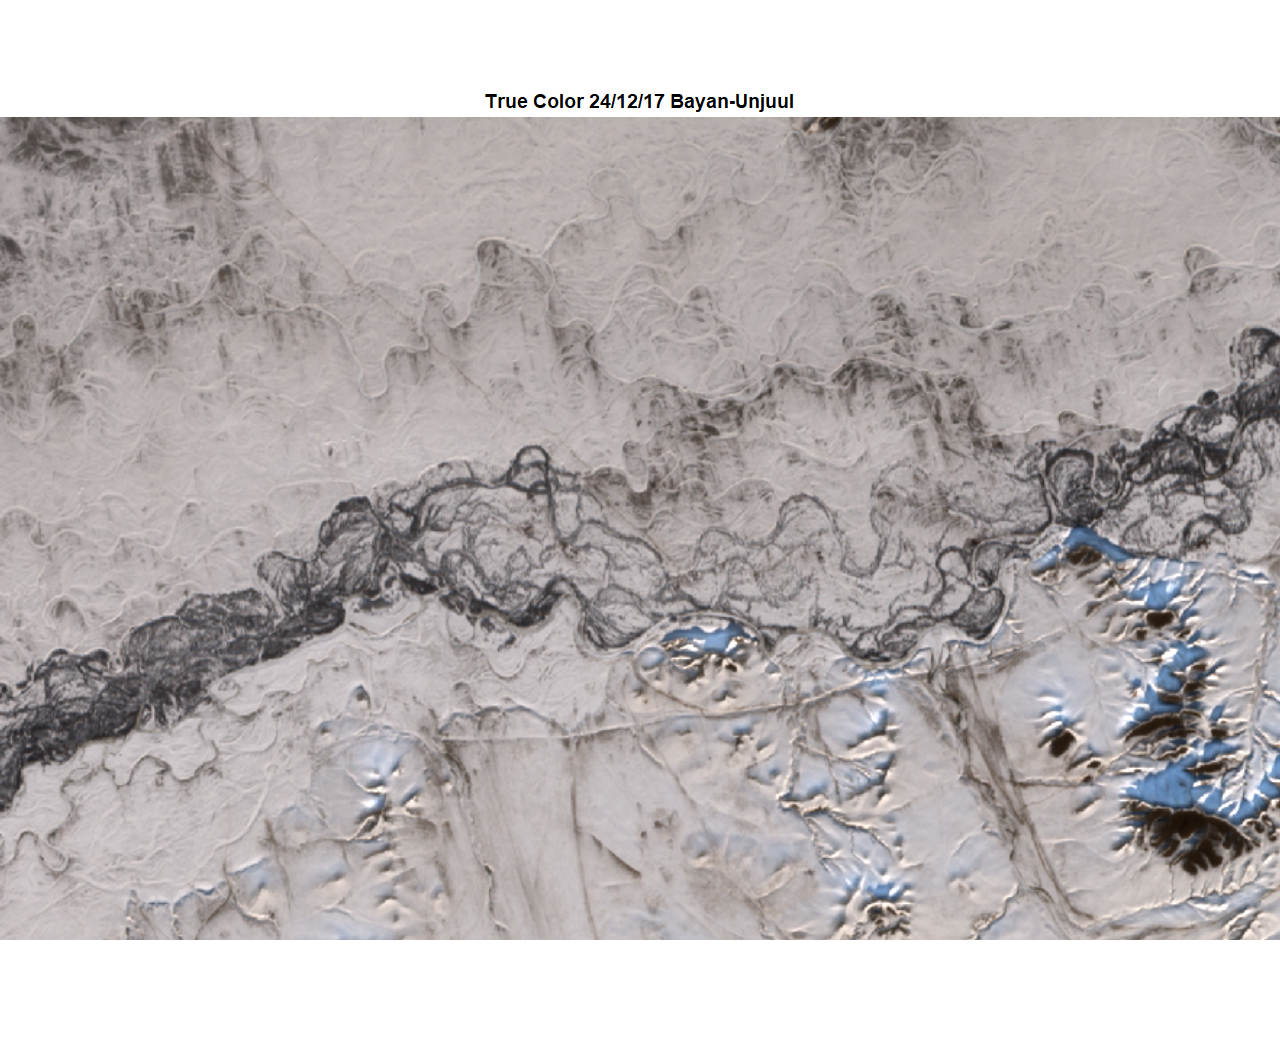
\includegraphics[width=\linewidth]{TC_17_Inv.png}
        \column{0.5\textwidth}
            \begin{itemize}
                \item<1-> True Color by RGB (red = b4, green = b3, blue = b2)
                \item<2-> Perennial snow troughtout the winter
                \item<3-> Frozen lakes and ponds
            \end{itemize}
    \end{columns}
\end{frame}
\begin{frame}[fragile]{True Color Script Example}
    \begin{lstlisting}[language=R]
#Carico il vettore contente le differenti bande
    
    true_color_2017 <- c(b4_17,b3_17,b2_17)

#Creo il plot RGB con rosso=b4,verde=b3,blu=b2
    
    tc_17 <- plotRGB(true_color_2017, 1, 2, 3, main = "True Color 24/12/17 Bayan-Unjuul")
    \end{lstlisting}
\end{frame}
\begin{frame}{Winter True Color Comparison}
    \centering
    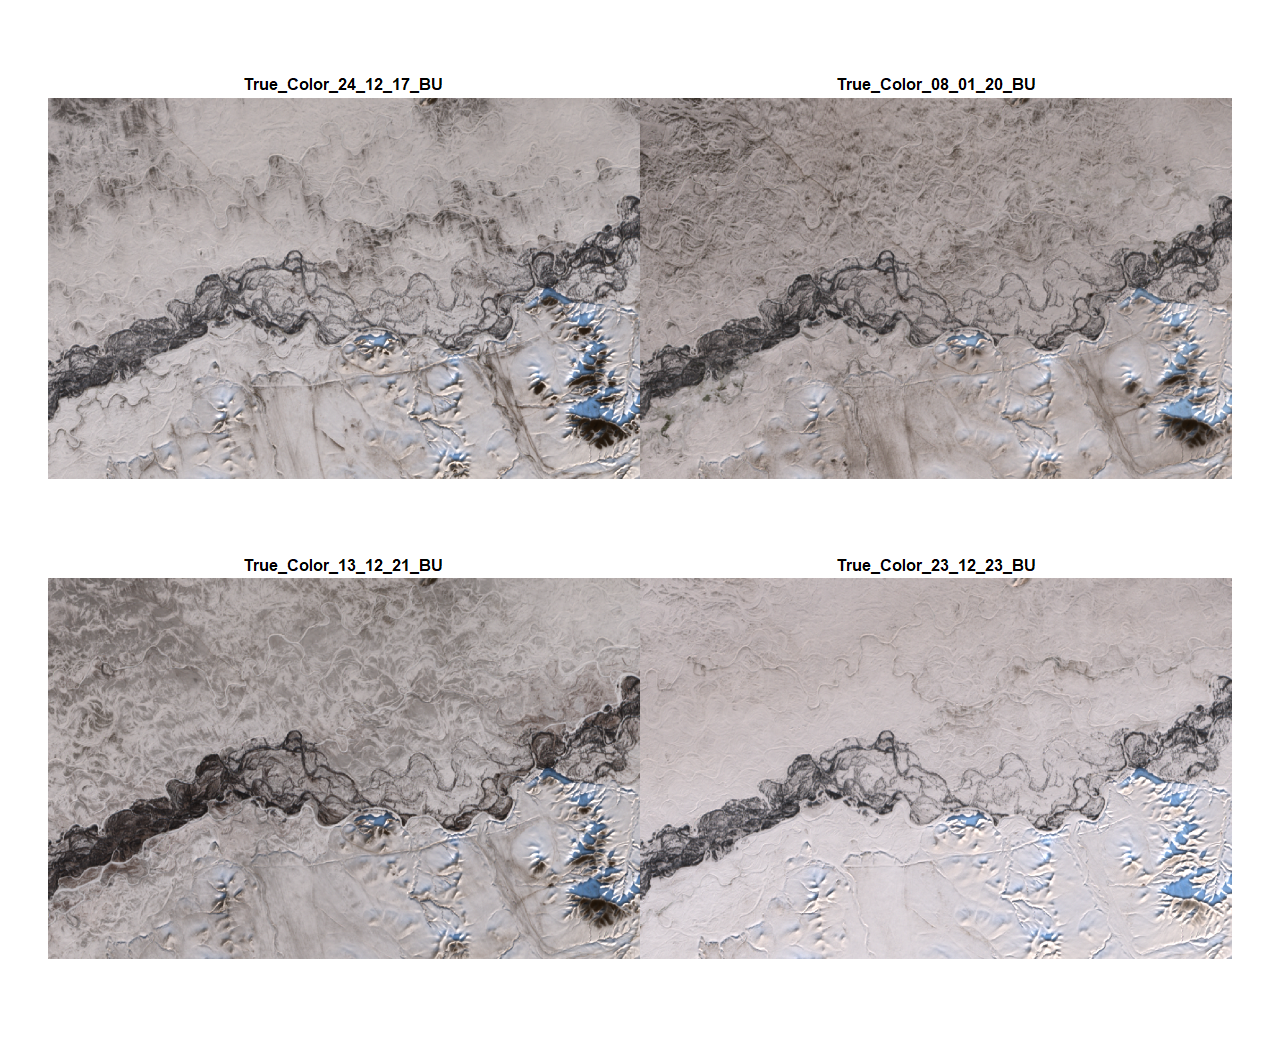
\includegraphics[width=0.9\textwidth]{Confronto_TC_Inv.png}  
\end{frame}
\begin{frame}[fragile]{True Color Script Example}
    \begin{lstlisting}[language=R]
#Dispongo i miei plot 2 per riga e su due colonne,
#Con oma() do dei margini dalla cornice rispetto i punti cardinali
    par(mfrow=c(2,2), oma=c(3,3,3,3))

    tc_17 <- plotRGB(true_color_2017, 1, 2, 3, main = "True_Color_24_12_17_BU")
    tc_20 <- plotRGB(true_color_2020, 1, 2, 3, main = "True_Color_08_01_20_BU")
    tc_21 <- plotRGB(true_color_2021, 1, 2, 3, main = "True_Color_13_12_21_BU")
    tc_23 <- plotRGB(true_color_2023, 1, 2, 3, main = "True_Color_23_12_23_BU")
    \end{lstlisting}
\end{frame}


\subsection{NDSI}
\begin{frame}{NDSI}
    \framesubtitle{To identify snow cover by distinguishing snow from other surfaces like clouds and water}
    \begin{columns}
        \column{0.5\textwidth}
            \textbf{Range:}
            \begin{itemize}
                \item +1 : Snow or Ice
                \item \hspace{0.8em}0 : Rocks, Sand
                \item \hspace{0.5em}-1 : Water
            \end{itemize}
            \vfill % This fills the vertical space to align with the other column
        \column{0.5\textwidth}
            \begin{itemize}
                \item   \[
                        NDSI = \frac{Green - SWIR}{Green + SWIR}
                        \]
                \item \small{SWIR: short-wave infrared light}
            \end{itemize}
            \vfill % This ensures the same height in the second column
    \end{columns}
\end{frame}

\begin{frame}[fragile]{NDSI Script Dec 2017}
    \begin{lstlisting}[language=R]
### NDSI 1 = NEVE/GHIACCIO , 0 = SUOLO  VEG, -1 = ACQUA O SIMILI ###    
## Palette colori ##

col_ndsi <- colorRampPalette(c("black", "brown", "white", "darkblue")) (100)

### 2017 ###

ndsi_2017 <- (b3_17 - b11_17) / (b3_17 + b11_17)
plot(ndsi_2017, col = col_ndsi, main = "NDSI 2017 Inverno")
    \end{lstlisting}
\end{frame}

\begin{frame}{NDSI Dec 2017}
    \centering
    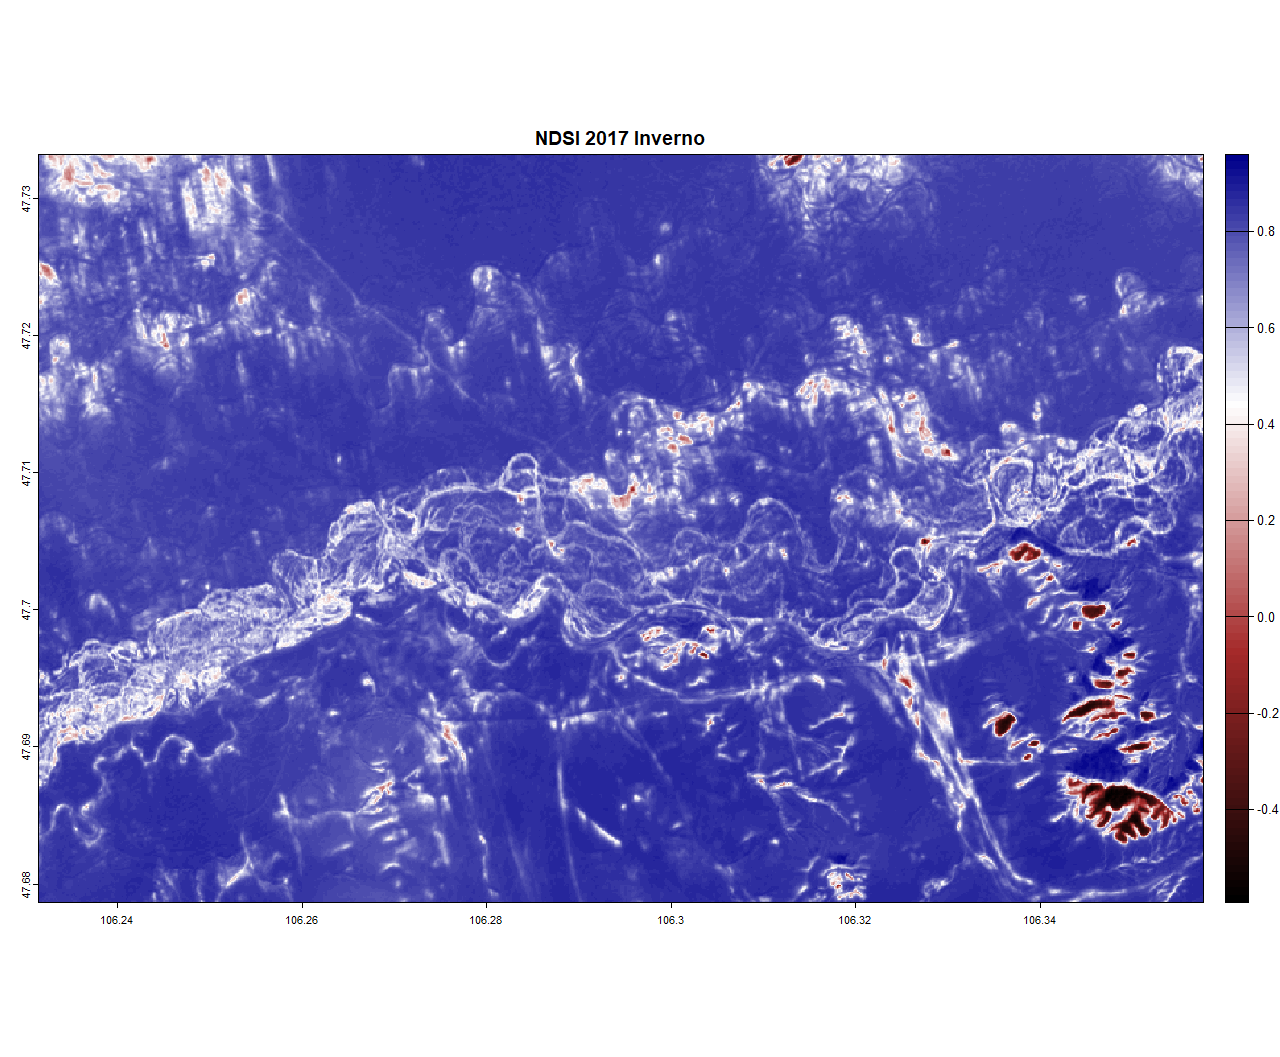
\includegraphics[width=0.9\textwidth]{NDSI_17_Inv.png}  
    
\end{frame}

\begin{frame}{NDSI Comparison}
    \centering
    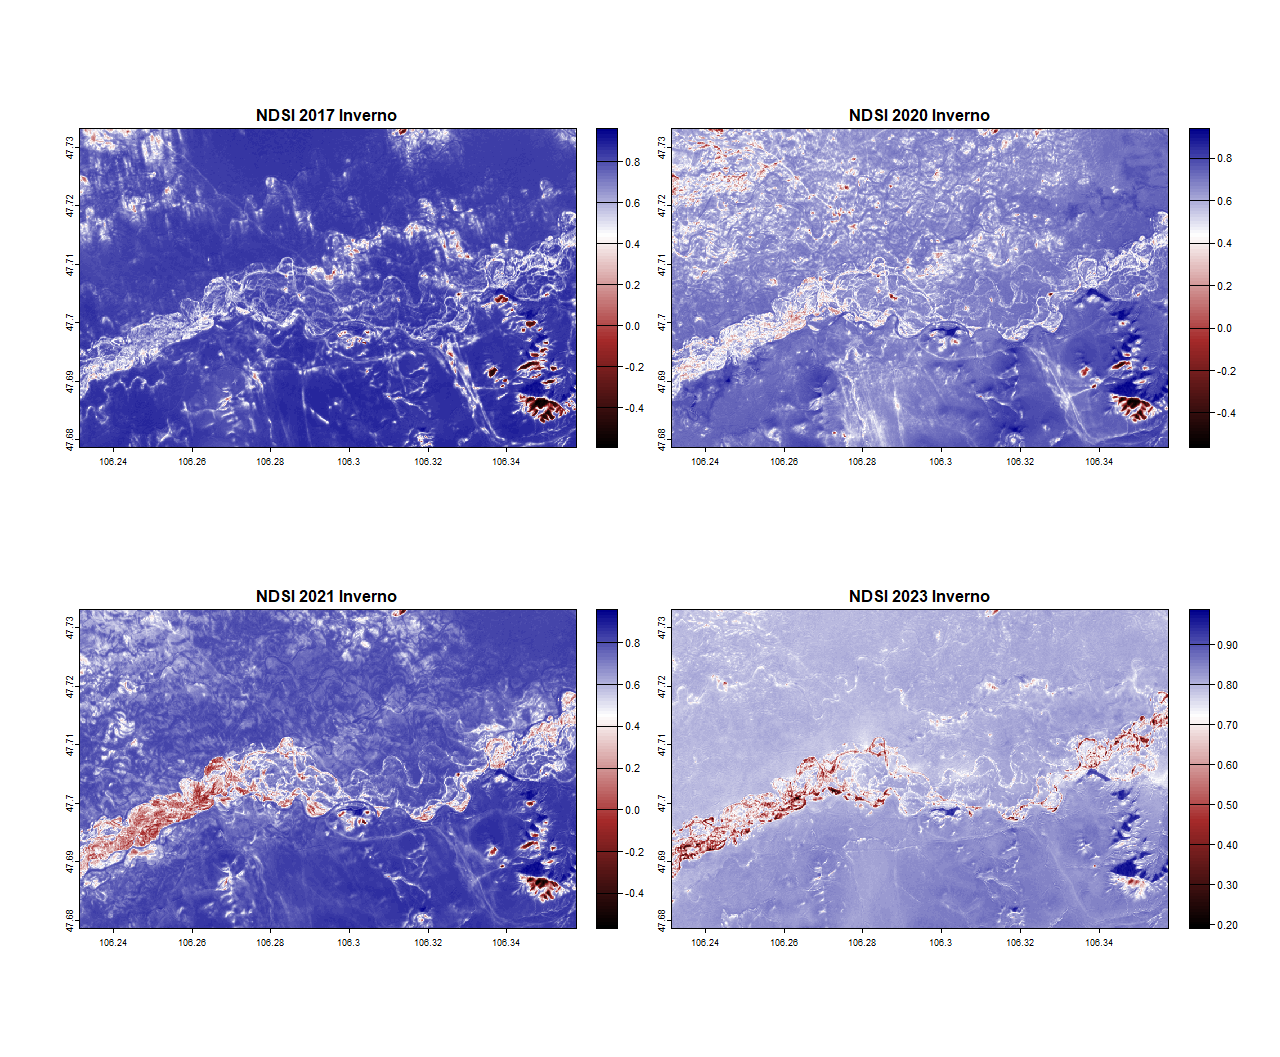
\includegraphics[width=0.9\textwidth]{Confronto_NDSI_Inv.png}
\end{frame}

\begin{frame}[fragile]{NDSI Comparison Script }
    \begin{lstlisting}[language=R]
#Confronto

par(mfrow=c(2,2), oma=c(3,3,3,3))

plot(ndsi_2017, col = col_ndsi, main = "NDSI 2017 Inverno")
plot(ndsi_2020, col = col_ndsi, main = "NDSI 2020 Inverno")
plot(ndsi_2021, col = col_ndsi, main = "NDSI 2021 Inverno")
plot(ndsi_2023, col = col_ndsi, main = "NDSI 2023 Inverno")

    \end{lstlisting}
\end{frame}

\begin{frame}{Standard Deviation}
\framesubtitle{Example: 2017}
    \centering
    \includegraphics[width=0.9\textwidth]{SD_17_Inv.png}
\end{frame}
\begin{frame}[fragile]{Standard Deviation Script}
    \begin{lstlisting}[language=R]
ndsi_sd_17 <- focal(ndsi_2017, w = matrix(1/169,13,13), fun = sd)
plot(ndsi_sd_17, col = col_ndsi, main = "Dev Stand 17")
    \end{lstlisting}
\end{frame}
\begin{frame}{Standard Deviation Comparison}
    \centering
    \includegraphics[width=0.9\textwidth]{Confronto_SD_inv.png}
\end{frame}

\begin{frame}{Plot Mean NDSI with SD (Standard Deviation)}
    \begin{columns}
        \column{0.7\textwidth}
            \only<1>{
                \includegraphics[width=\linewidth]{plot_mean_sd_Inv.png}
            }
            \only<2>{
                \includegraphics[width=\linewidth]{SD_PLOT_red_Inv.png}
            }
        \column{0.3\textwidth} 
            \begin{itemize}
                \item<1->No significant variation for the years 2017, 2020, and 2021.
                \item<2->Lower NDSI value in 2023.
            \end{itemize}
    \end{columns}
    
\end{frame}

\begin{frame}{PCA (Principal Component Analysis)}
    \begin{columns}
        \column{0.7\textwidth}
            \includegraphics[width=\linewidth]{PCA_Inv.png}

        \column{0.3\textwidth} 
            \begin{itemize}
                \item  PC1: Strong contrast between lighter (yellow) and darker (purple) areas, likely indicating regions with the most significant NDSI variations 
                \item PC2 - PC3: No significant variations captured
            \end{itemize}
    \end{columns}
    
\end{frame}




\section{Summer}
\subsection{TrueColor}
\begin{frame}{Summer}
    \framesubtitle{June 2017}
        \centering
        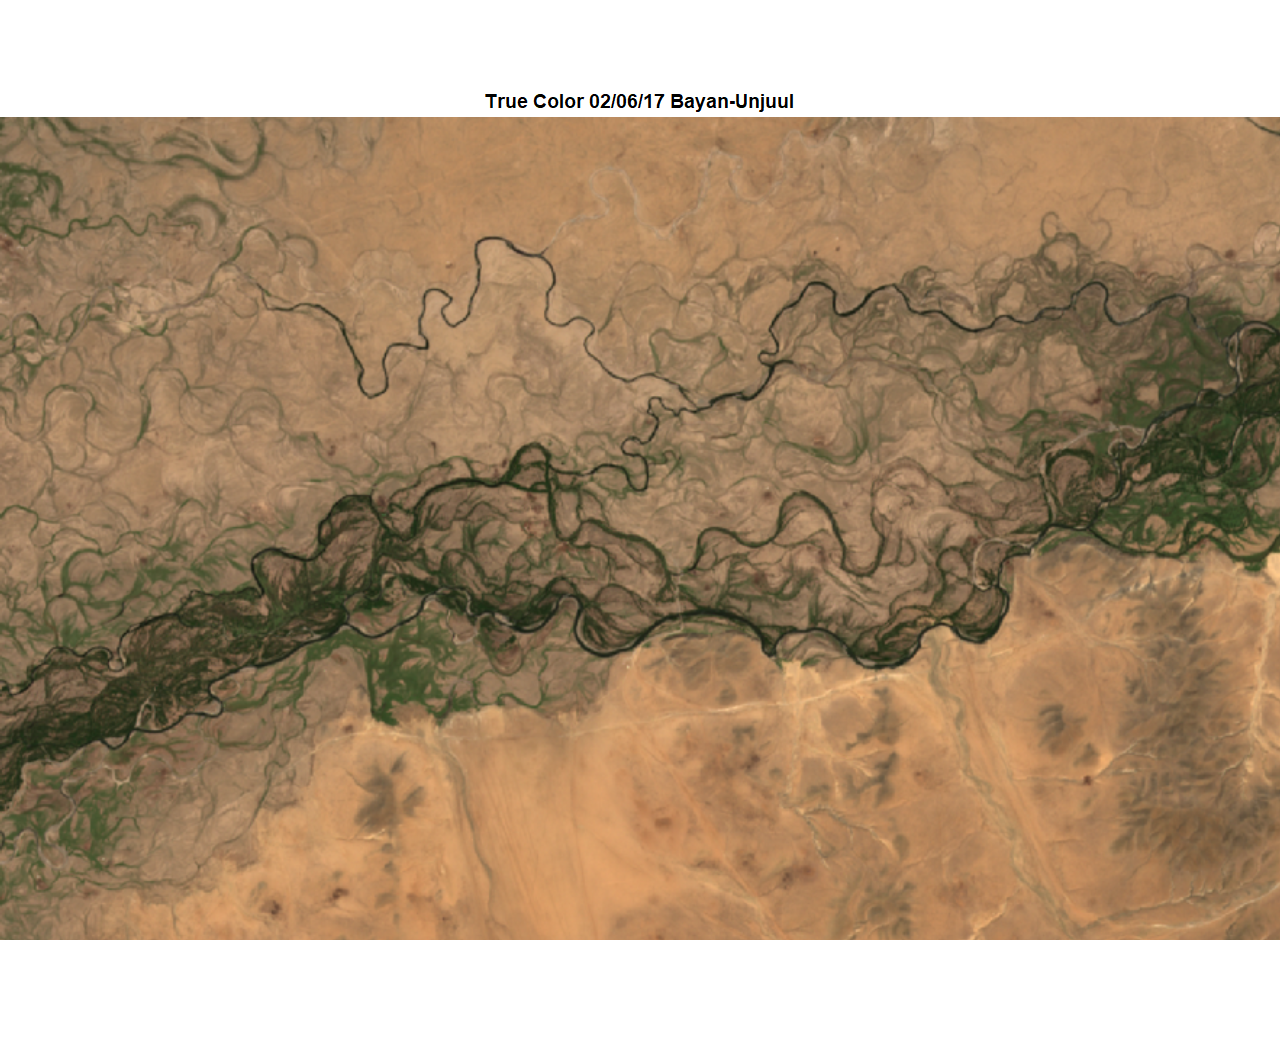
\includegraphics[width=0.9\textwidth]{TC_17_Sum.png}
\end{frame}

\begin{frame}{Summer True Color Comparison}
    \centering
    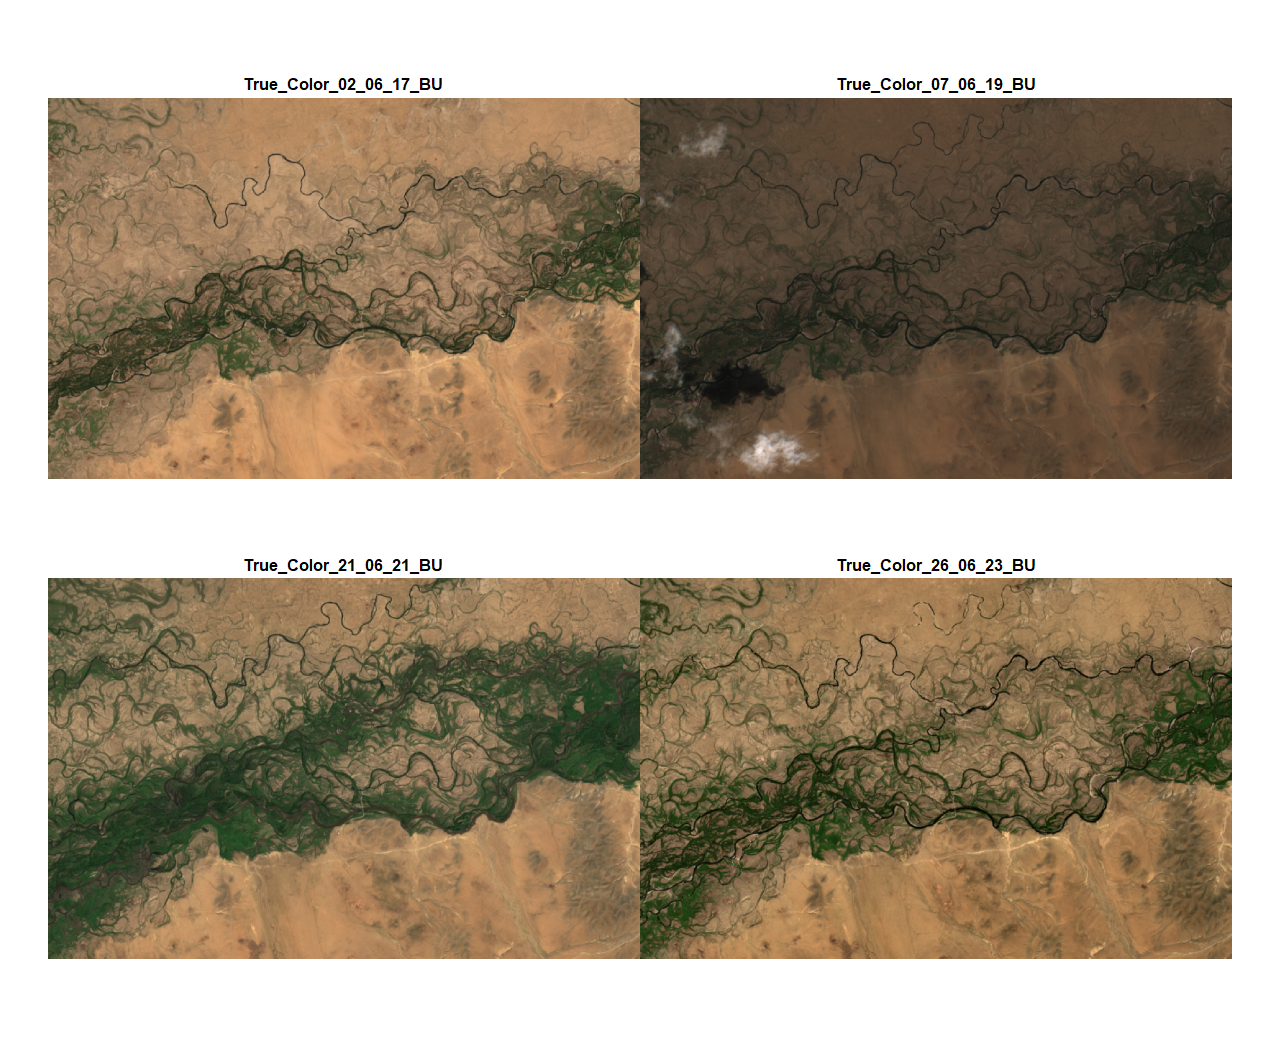
\includegraphics[width=0.9\textwidth]{Confronto_TC_Sum.png}  
\end{frame}

\subsection{NDVI}
\begin{frame}{NDVI (Normalized Difference Vegetation Index))}
    \framesubtitle{Index that measures the density and health of vegetation}
    \begin{columns}
        \column{0.5\textwidth}
            \textbf{Range:}
            \begin{itemize}
                \item +1 :  Dense, healthy vegetation
                \item \hspace{0.8em}0 : Sparse vegetation or soil
                \item \hspace{0.5em}-1 : Non-vegetated surfaces like water, snow, or ice
            \end{itemize}
            \vfill % This fills the vertical space to align with the other column
        \column{0.5\textwidth}
            \begin{itemize}
                \item   \[
                        NDVI = \frac{NIR(b8) - Red(b4)}{NIR(b8) + Red(b4)}
                        \]
                \item \small{NIR: near-infrared band, vegetation strongly reflects.}
            \end{itemize}
            \vfill % This ensures the same height in the second column
    \end{columns}
\end{frame}

\begin{frame}[fragile]{NDVI Script Dec 2017}
    \begin{lstlisting}[language=R]
### NDVI 1 = temperate/tropicali ; 0.2 - 0.4 = shrub/grassland ; -0.1 - 0.1 = roccia, sabbia, neve ; -1 = acqua ###

## Palette colori ##

col_ndvi <- colorRampPalette(c("black", "grey", "green", "darkgreen")) (100)

### 2017 ###
ndvi_2017_g <- (b8_17_ndvi - b4_17_ndvi) / (b8_17_ndvi + b4_17_ndvi)
plot(ndvi_2017_g, col = col_ndvi, main = "NDVI 2017 Giugno")
    \end{lstlisting}
\end{frame}

\begin{frame}{NDVI Jun 2017}
    \centering
    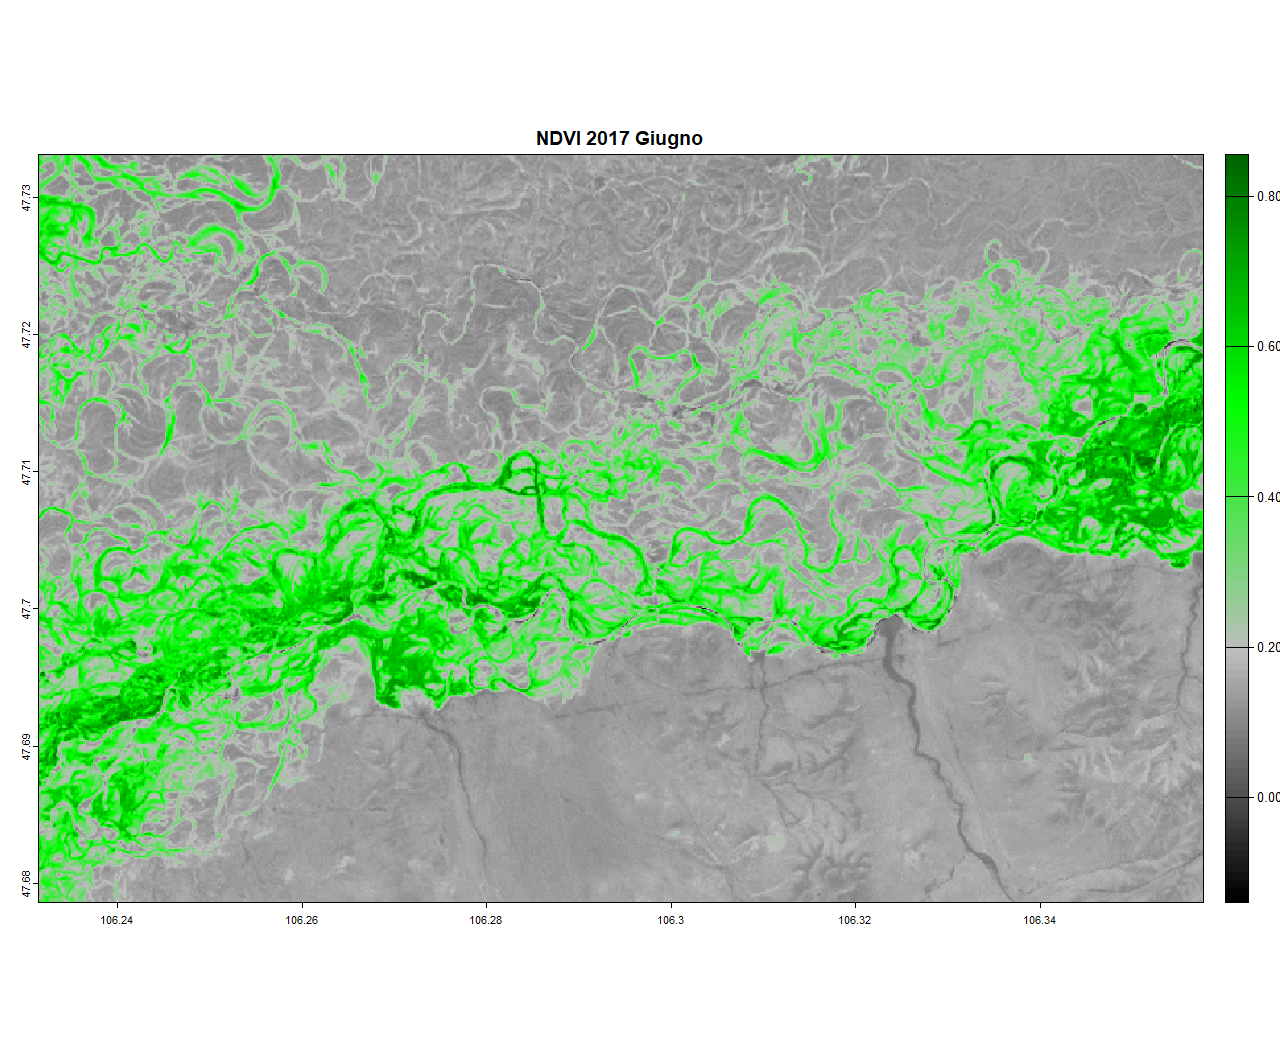
\includegraphics[width=0.9\textwidth]{NDVI_17_Sum.png}  
    
\end{frame}

\begin{frame}{NDVI Comparison}
    \centering
    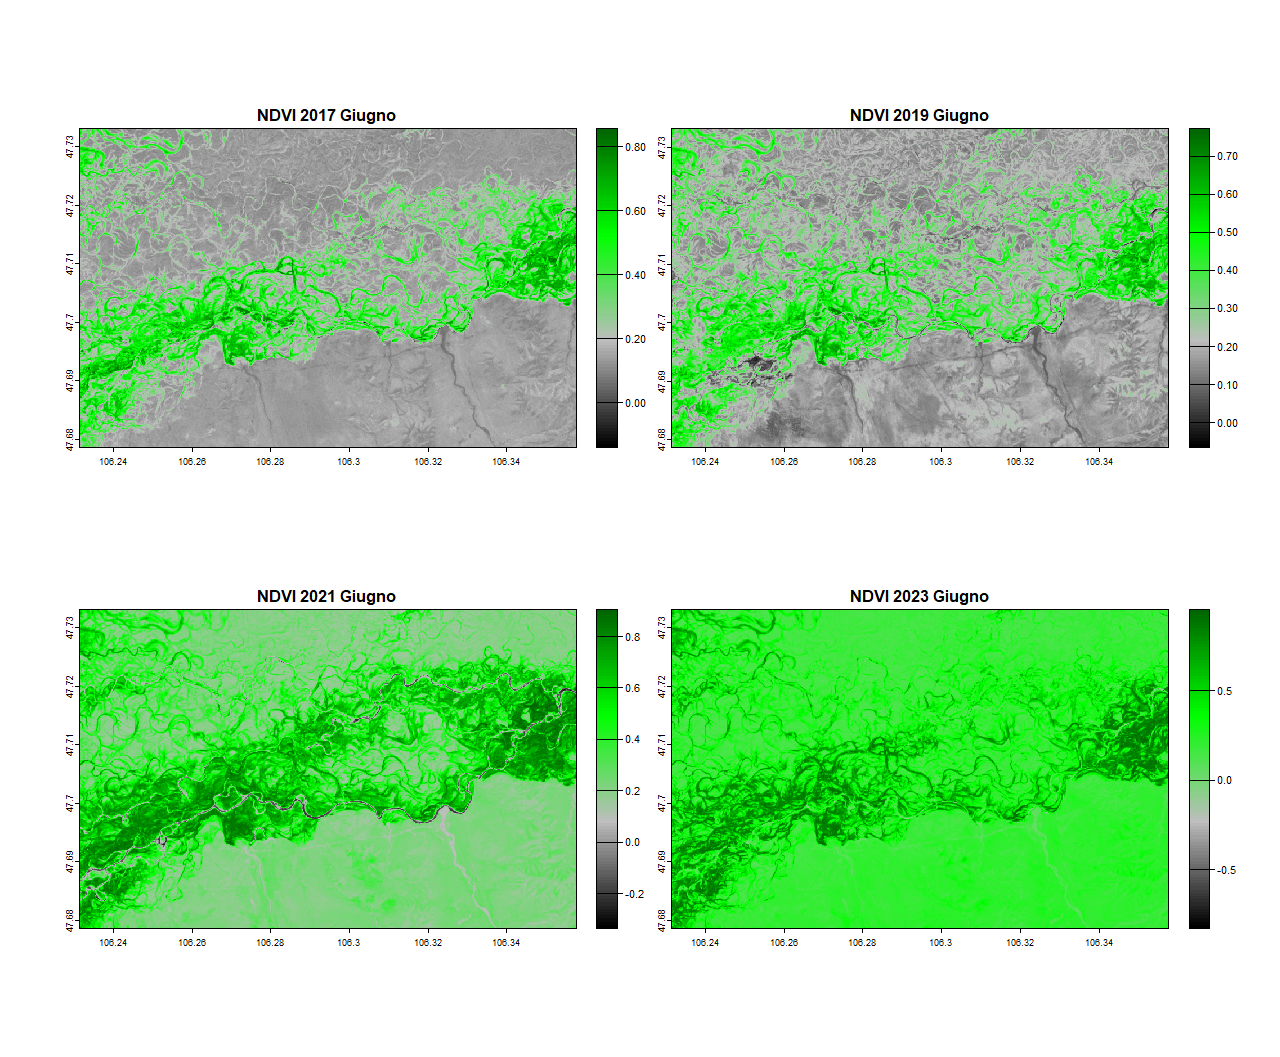
\includegraphics[width=0.9\textwidth]{Confronto_NDVI_Sum.png}
\end{frame}


\begin{frame}{Standard Deviation}
\framesubtitle{Summer Standard Deviation Comparison}
    \centering
    \includegraphics[width=0.9\textwidth]{Comparison_sd_Sum.png}
\end{frame}


\begin{frame}{Plot Mean NDVI with SD (Standard Deviation)}
    \begin{columns}
        \column{0.7\textwidth}
            \only<1>{
                \includegraphics[width=\linewidth]{sd_plot_Sum_1.png}
            }
            \only<2>{
                \includegraphics[width=\linewidth]{sd_plot_sum_2.png}
            }
        \column{0.3\textwidth} 
            \begin{itemize}
                \item<1->No variations between 2017 - 2019
                \item<2->Higher values of NDVI in 2021 - 2023.
            \end{itemize}
    \end{columns}
    
\end{frame}


\begin{frame}{PCA (Principal Component Analysis) NDVI}
    \begin{columns}
        \column{0.7\textwidth}
            \includegraphics[width=\linewidth]{PCA_Summer_NDVI.png}

        \column{0.3\textwidth} 
            \begin{itemize}
                \item PC1: There are clear patterns, possibly representing rivers, forests, or dense vegetation areas 
                \item PC2: Might reflect inter-annual variations in vegetation
                \item PC3: Captures residual variation that isn’t as visually significant
            \end{itemize}
    \end{columns}
    
\end{frame}
\subsection{NDMI}
\begin{frame}{NDMI (Normalized Difference Moisture Index))}
    \framesubtitle{Index used to assess vegetation moisture content, especially in relation to soil and plant water stress}
    \begin{columns}
        \column{0.5\textwidth}
            \textbf{Range:}
            \begin{itemize}
                \item +1 :  High moisture content, typically seen in well-hydrated, healthy vegetation.
                \item \hspace{0.8em}0 : Lower vegetation moisture or dry conditions
                \item \hspace{0.5em}-1 : Very dry conditions
            \end{itemize}
            \vfill % This fills the vertical space to align with the other column
        \column{0.5\textwidth}
            \begin{itemize}
                \item   \[
                        NDMI = \frac{NIR(b8A) - SWIR(b11)}{NIR(b8A) - SWIR(b11)}
                        \]
            \end{itemize}
            \vfill % This ensures the same height in the second column
    \end{columns}
\end{frame}

\begin{frame}[fragile]{NDMI Script June 2017}
    \begin{lstlisting}[language=R]
## Palette colori ##

col_ndmi <- colorRampPalette(c("black", "white", "red", "darkred")) (100)

#NDMI#
ndmi_2017_g <- (b8a_17_g - b11_17_g) / (b8a_17_g + b11_17_g)
    \end{lstlisting}
\end{frame}

\begin{frame}{NDMI June 2017}
    \centering
    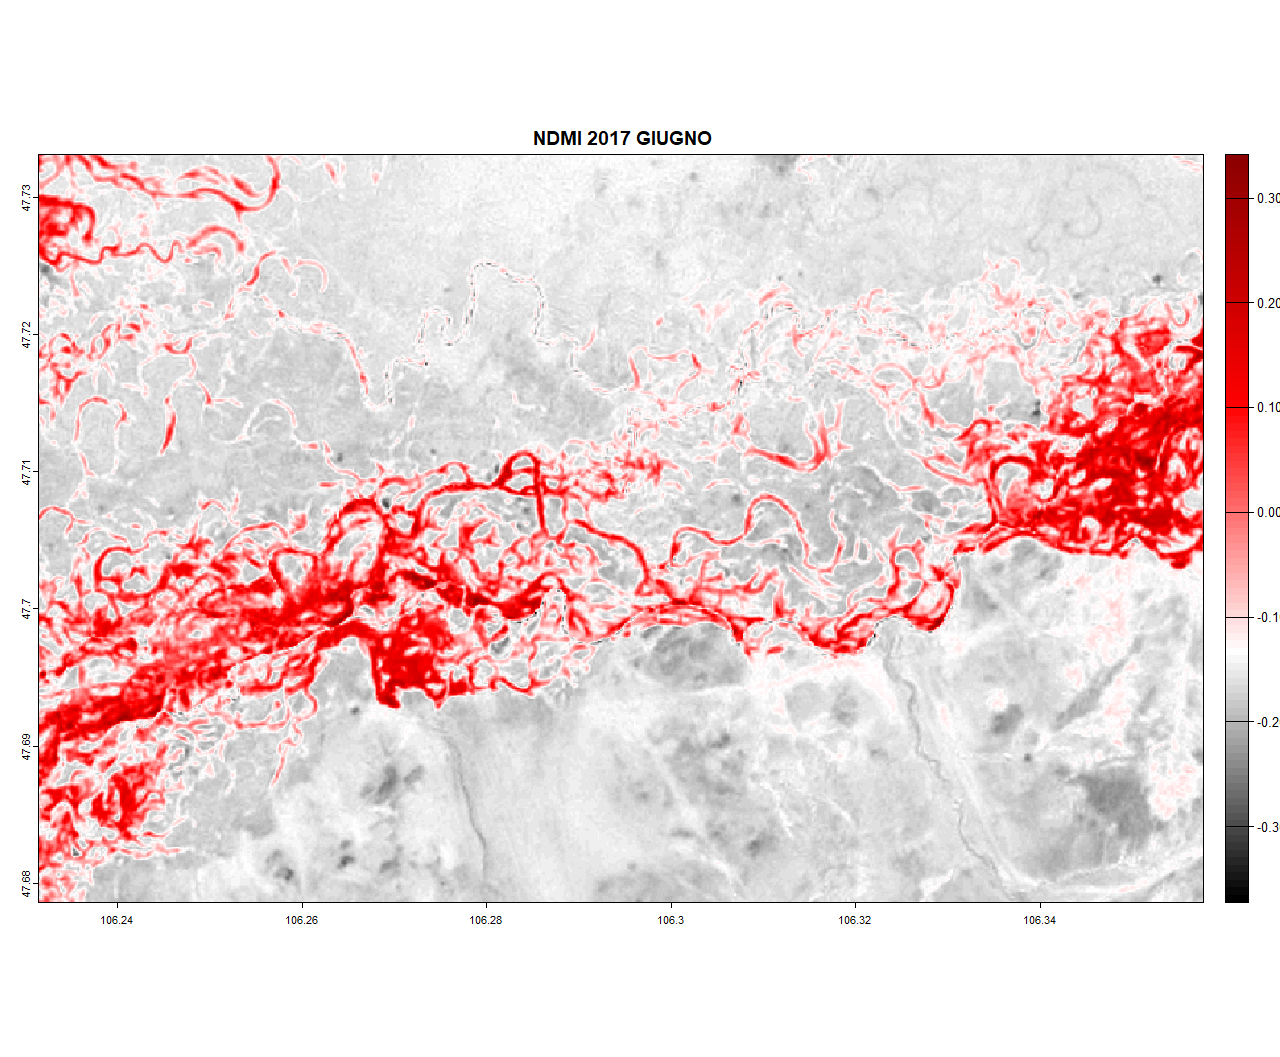
\includegraphics[width=0.9\textwidth]{NDMI_17_Sum.png}  
    
\end{frame}

\begin{frame}{NDMI Comparison}
    \centering
    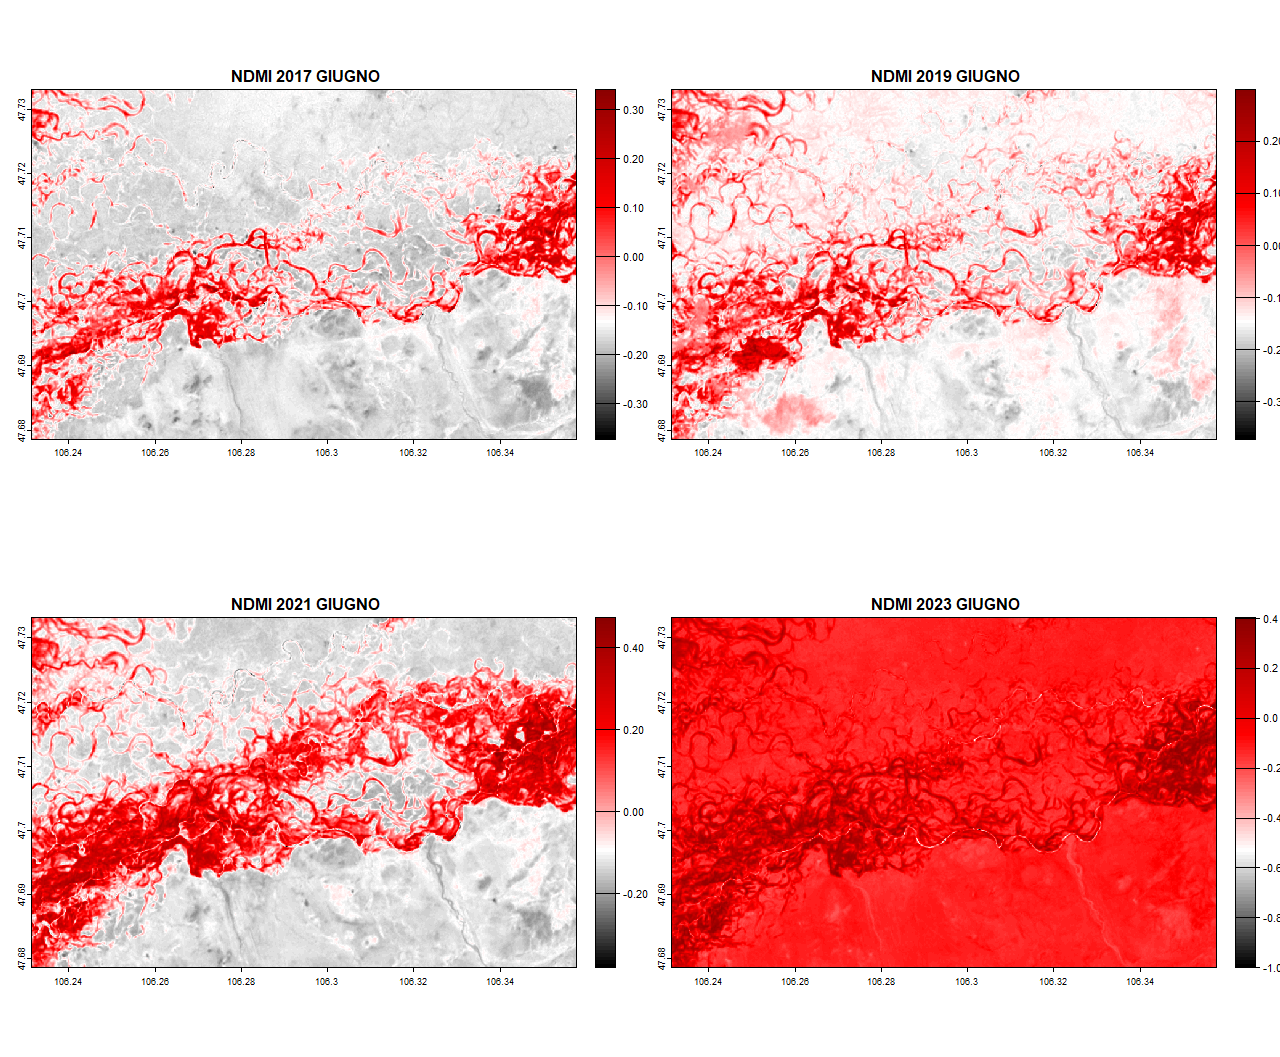
\includegraphics[width=0.9\textwidth]{Confronto_NDMI_Sum.png}
\end{frame}

\begin{frame}{Standard Deviation}
\framesubtitle{Summer Standard Deviation Comparison}
    \centering
    \includegraphics[width=0.9\textwidth]{Confronto_NDMI_SD_Sum.png}
\end{frame}


\begin{frame}{Plot Mean NDMI with SD (Standard Deviation)}
    \begin{columns}
        \column{0.7\textwidth}
            \only<1>{
                \includegraphics[width=\linewidth]{sd_plot_ndmi_sum_1.png}
            }
            \only<2>{
                \includegraphics[width=\linewidth]{sd_plot_ndmi_sum_2.png}
            }
        \column{0.3\textwidth} 
            \begin{itemize}
                \item<1->No variations between 2017 - 2019
                \item<2->Higher values of NDVI in 2021 - 2023.
            \end{itemize}
    \end{columns}
    
\end{frame}

\begin{frame}{PCA (Principal Component Analysis) NDMI}
    \begin{columns}
        \column{0.7\textwidth}
            \includegraphics[width=\linewidth]{pca_ndmi_sum.png}

        \column{0.3\textwidth} 
            \begin{itemize}
                \item PC1: There are clear patterns, possibly representing rivers, forests, or dense vegetation areas 
                \item PC2: Might reflect inter-annual variations in vegetation
                \item PC3: Captures residual variation that isn’t as visually significant
            \end{itemize}
    \end{columns}
    
\end{frame}
\section{Spring}
\subsection{TrueColor}
\begin{frame}{Spring}
    \framesubtitle{April 2017}
        \centering
        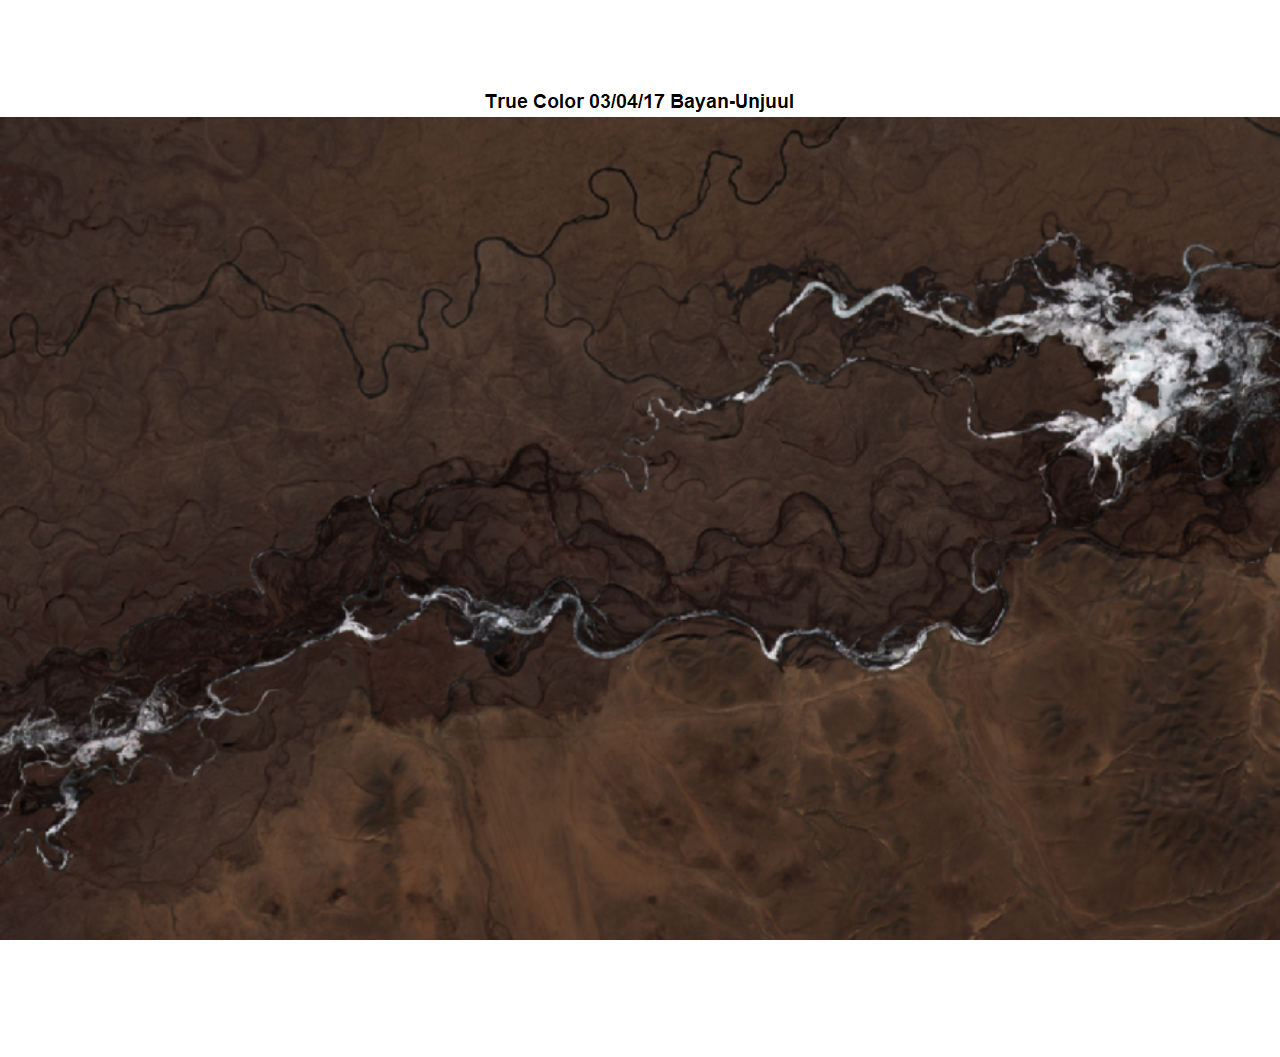
\includegraphics[width=0.9\textwidth]{TC_17_Spr.png}
\end{frame}

\begin{frame}{Spring True Color Comparison}
    \centering
    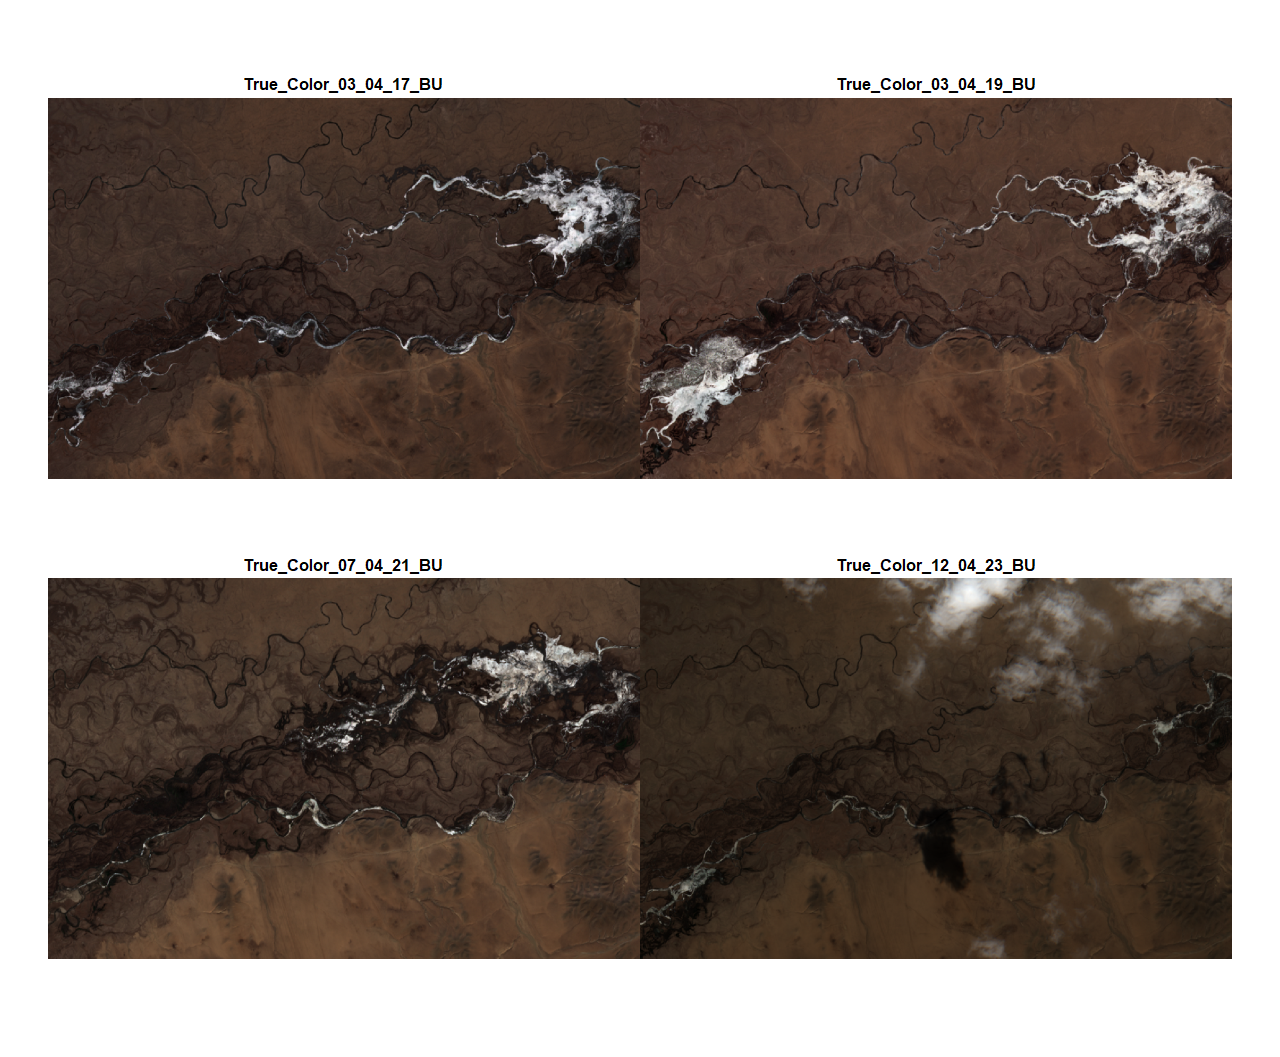
\includegraphics[width=0.9\textwidth]{Confronto_TC_Spr.png}  
\end{frame}

\subsection{NDVI}
\begin{frame}{NDVI April 2017}
    \centering
    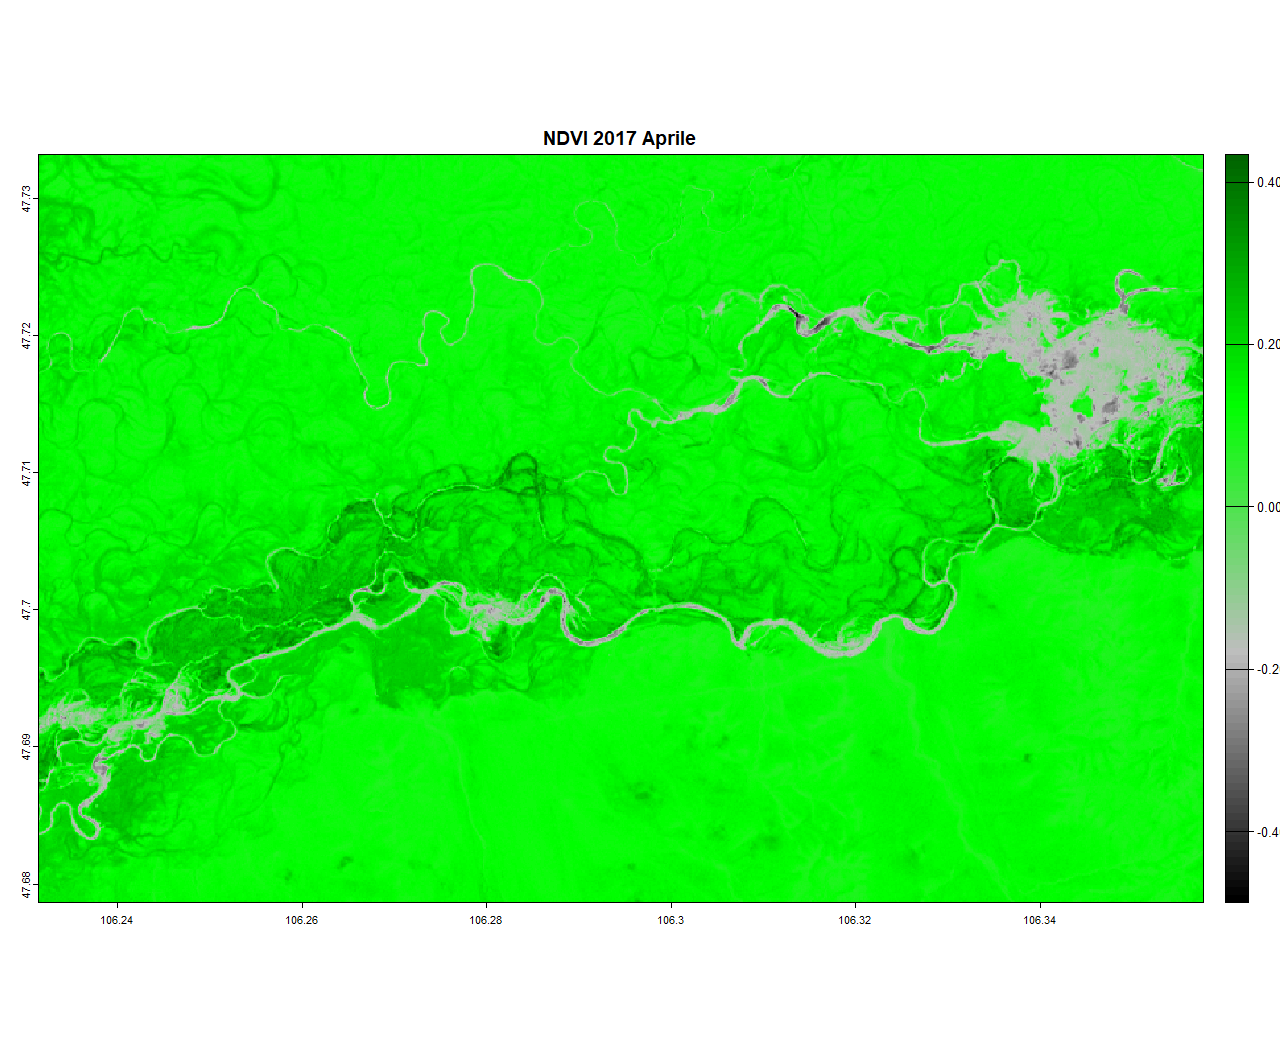
\includegraphics[width=0.9\textwidth]{NDVI_17_Spr.png}  
    
\end{frame}

\begin{frame}{NDVI Comparison}
    \centering
    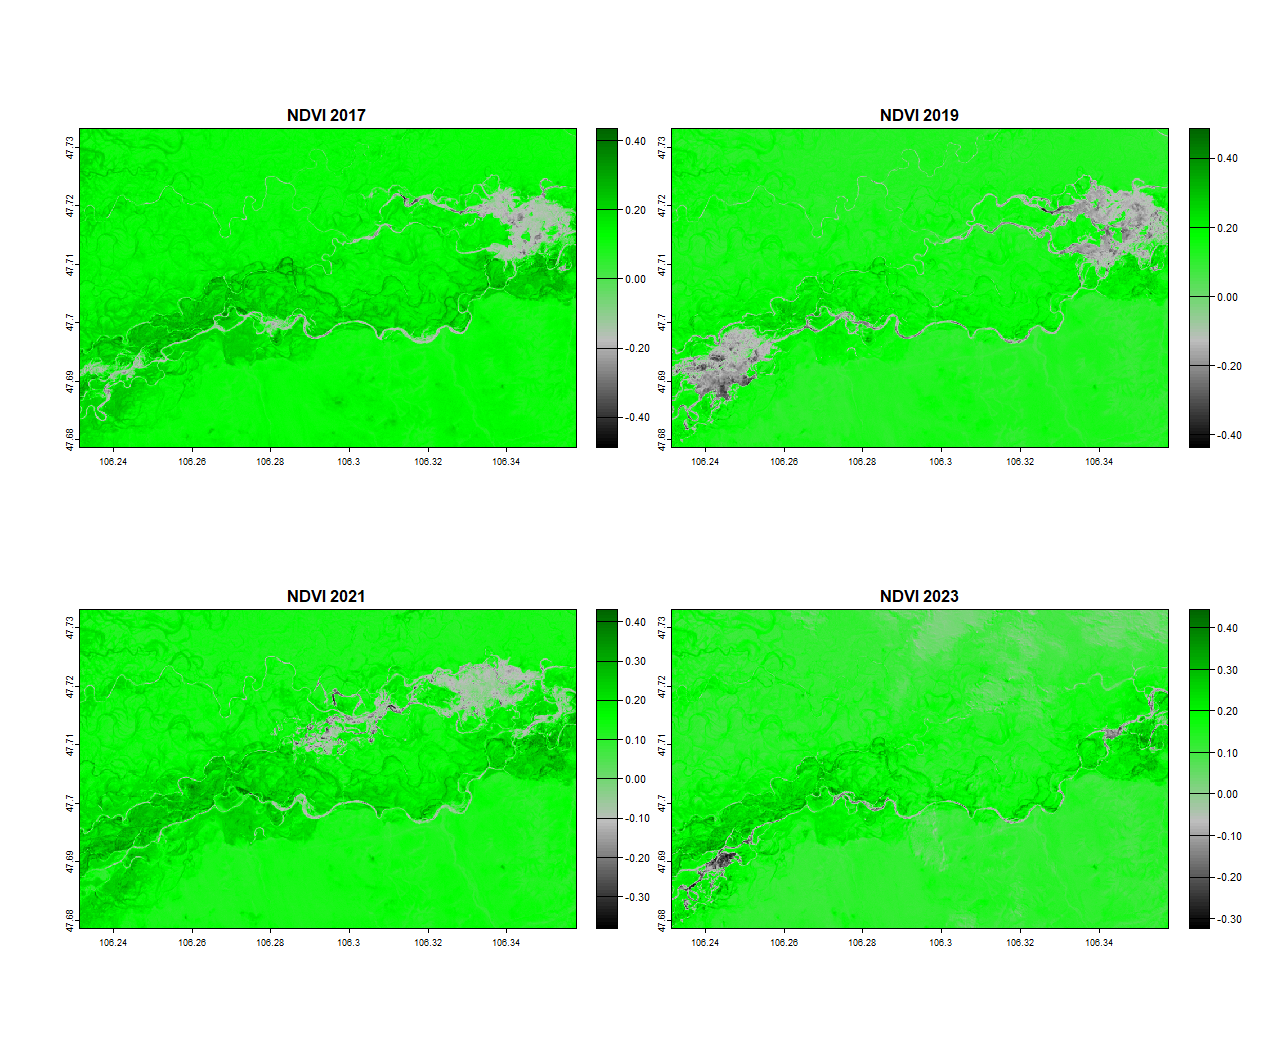
\includegraphics[width=0.9\textwidth]{Confronto_NDVI_Spr.png}
\end{frame}

\begin{frame}{Standard Deviation}
\framesubtitle{Spring Standard Deviation Comparison}
    \centering
    \includegraphics[width=0.9\textwidth]{SD_SPRING_COMPARISON.png}
\end{frame}


\begin{frame}{Plot Mean NDVI with SD (Standard Deviation)}
    \begin{columns}
        \column{0.7\textwidth}
                \includegraphics[width=\linewidth]{Plot_NDVI_MEAN_SD_Spr.png}
        \column{0.3\textwidth} 
            \begin{itemize}
                \item<1->No relevant variations except lower NDVI values for 2023
            \end{itemize}
    \end{columns}
    
\end{frame}

\begin{frame}{PCA (Principal Component Analysis) NDVI}
    \begin{columns}
        \column{0.7\textwidth}
            \includegraphics[width=\linewidth]{PCA_NDVI_Spr.png}

        \column{0.3\textwidth} 
            \begin{itemize}
                \item PC1: There are clear patterns, possibly representing rivers, forests, or dense vegetation areas 
                \item PC2: Might reflect inter-annual variations in vegetation
                \item PC3: Captures residual variation that isn’t as visually significant
            \end{itemize}
    \end{columns}
    
\end{frame}
\subsection{NDMI}

\begin{frame}{NDMI April 2017}
    \centering
    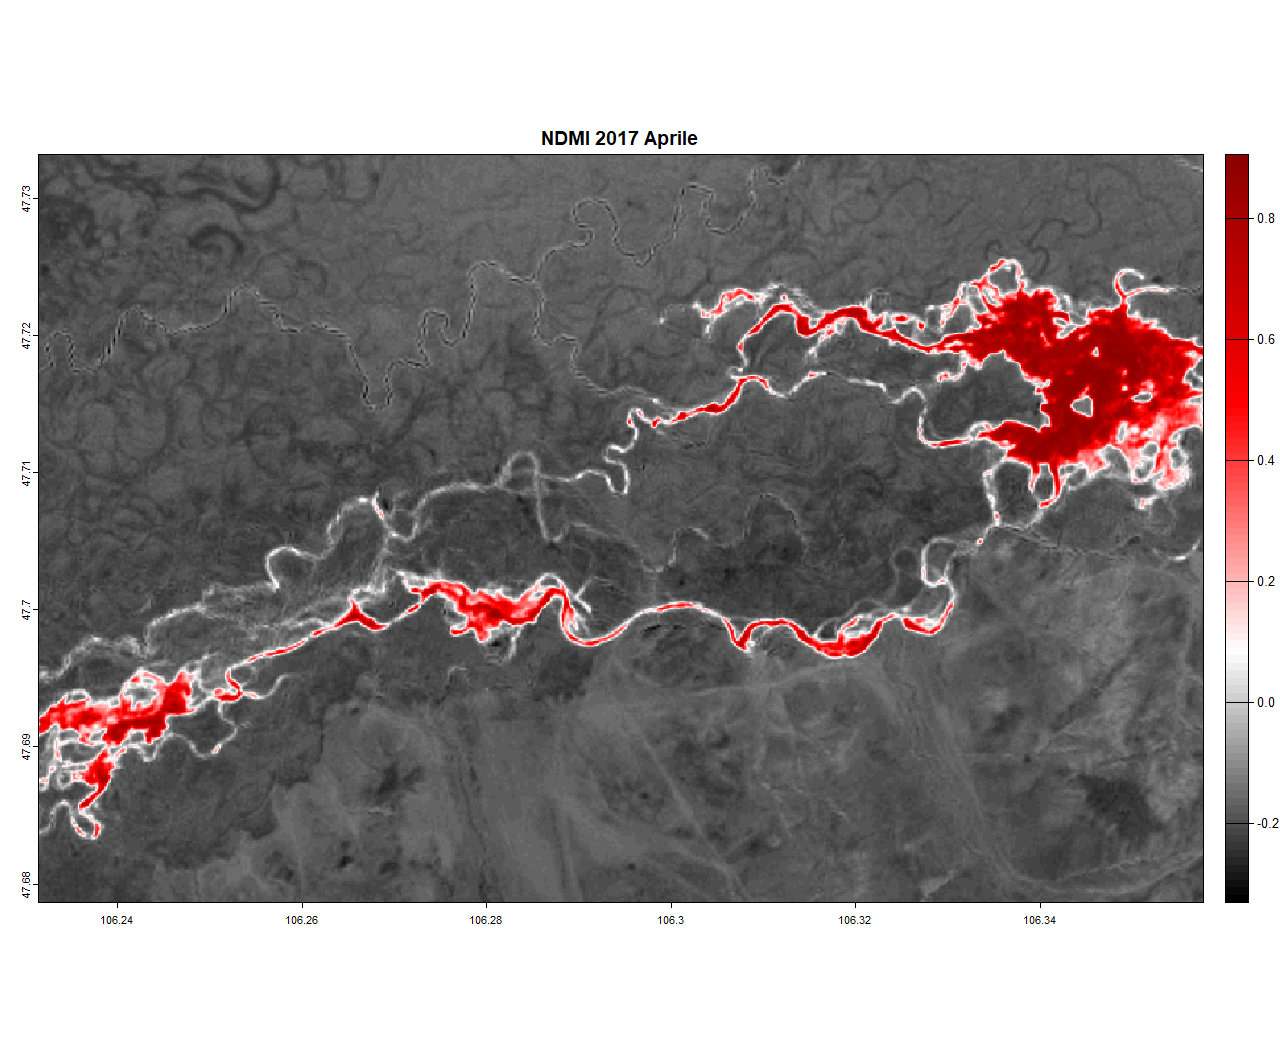
\includegraphics[width=0.9\textwidth]{NDMI_17_Spr.png}  
    
\end{frame}

\begin{frame}{NDMI Comparison}
    \centering
    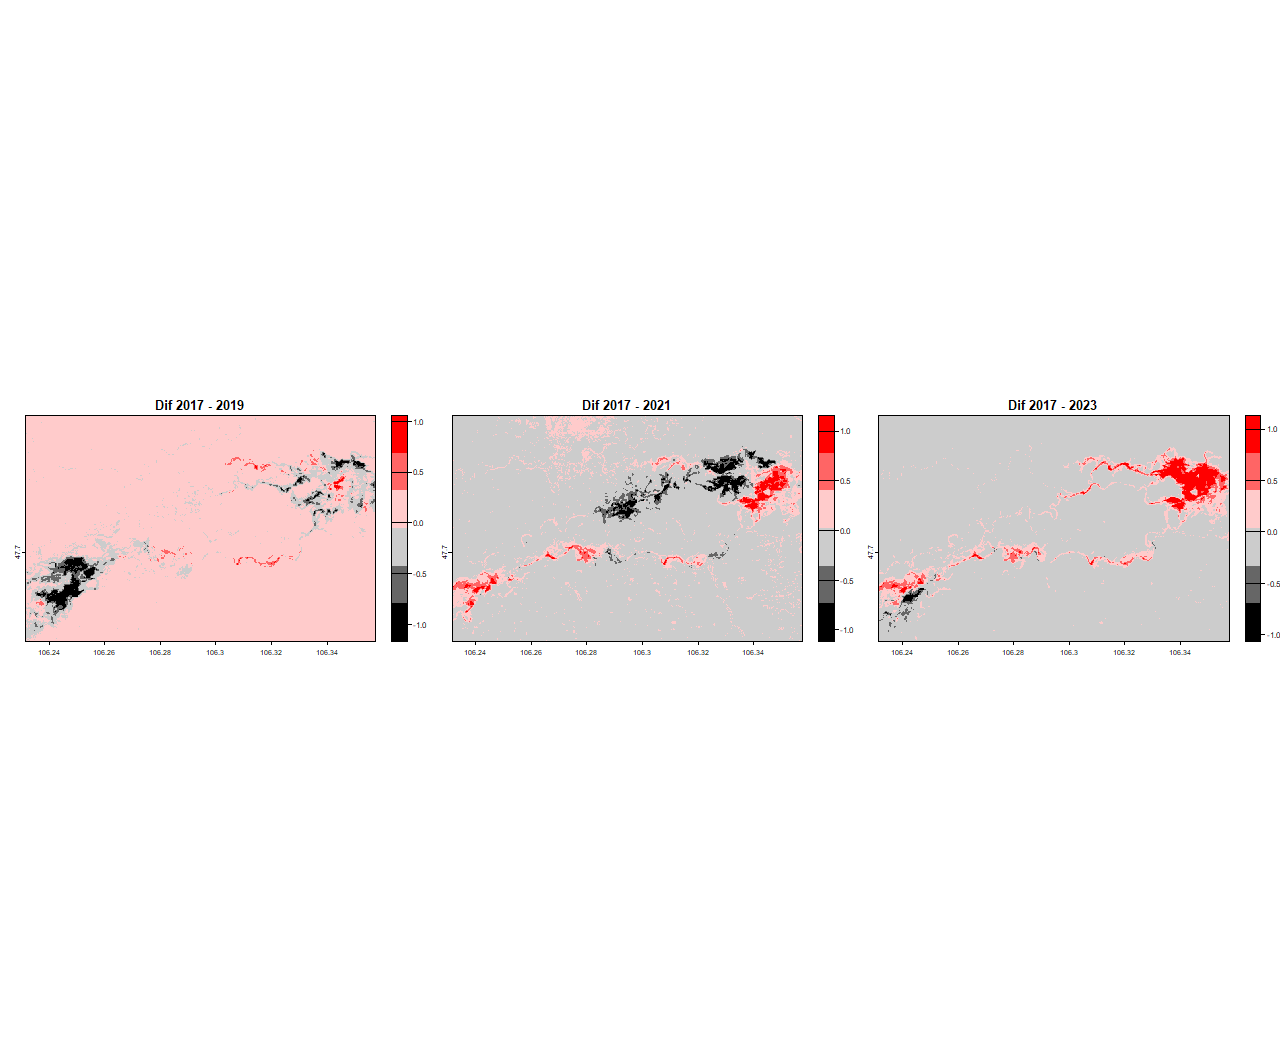
\includegraphics[width=0.9\textwidth]{Confronto_NDMI_Spr.png}
\end{frame}

\begin{frame}{Standard Deviation}
\framesubtitle{Spring Standard Deviation Comparison}
    \centering
    \includegraphics[width=0.9\textwidth]{SD_SPRING_COMPARISON_ndmi.png}
\end{frame}


\begin{frame}{Plot Mean NDMI with SD (Standard Deviation)}
    \begin{columns}
        \column{0.7\textwidth}
            \only<1>{
                \includegraphics[width=\linewidth]{Plot_NDMI_SPR.png}
            }
            \only<2>{
                \includegraphics[width=\linewidth]{Plot_ndmi_Spr_2.png}
            }
        \column{0.3\textwidth} 
            \begin{itemize}
                \item<1->No variations between 2017 - 2019 - 2021
                \item<2->Lower values of NDMI in 2023.
            \end{itemize}
    \end{columns}
    
\end{frame}

\begin{frame}{PCA (Principal Component Analysis) NDMI}
    \centering
    \includegraphics[width=0.9\linewidth]{PCA_NDMI_SPr.png}
\end{frame}

\section{Conclusions}
\begin{frame}{Observations}
    \begin{itemize}
        \item \textbf{NDSI Analysis:} Show a decrease in snow coverage over the years, which can have significant impacts on the ecosystem.
        \item \textbf{NDMI Spring Analysis:} Less snow leads to earlier melting and reduced soil water availability in spring.
        \item \textbf{NDVI Summer Analysis:} Despite the decrease in snow coverage and reduced soil moisture, an increase in vegetation is observed during summer. Moderate Water Stress (NDMI)
    \end{itemize}
\end{frame}

\begin{frame}{Conclusions}
    \begin{itemize}
        \item The \textbf{decrease} in snow and the resulting changes in the water cycle highlight the importance of monitoring the effects of climate change on water resource availability and vegetation.
        \item Understanding these dynamics is \textbf{crucial} for implementing sustainable natural resource management strategies.
    \end{itemize}
\end{frame}


\end{document}

